\documentclass[a4paper,12pt,oneside,pdflatex,italian,final,twocolumn]{article}

\usepackage[utf8]{inputenc}
\usepackage{parallel}
\usepackage{siunitx}
\usepackage{booktabs}
\usepackage{fancyhdr}
\usepackage{subcaption}
\usepackage{minted}
\usepackage{hyperref}
\usepackage{pdfpages}

\usepackage[export]{adjustbox}
\usepackage[margin=0.5in]{geometry}
\addtolength{\topmargin}{0in}

\usepackage{libertine}
\renewcommand*\familydefault{\sfdefault}  %% Only if the base font of the document is to be sans serif
\usepackage[T1]{fontenc}

\hypersetup{
	colorlinks=true, %set true if you want colored links
	linktoc=all,     %set to all if you want both sections and subsections linked
	linkcolor=blue,  %choose some color if you want links to stand out
	urlcolor=blue,   %url color
}

\definecolor{LightGray}{gray}{0.95}

\title{Custom Vibration Sensor v0}
\author{Achmadi ST MT}
\date{September 2023}

\begin{document}
	\pagestyle{fancy}

	\lhead{Achmadi ST MT}
	\chead{\today}
	\rhead{Specification Document}

	\onecolumn
	\begin{figure}

	\end{figure}\begin{minipage}{0.47\textwidth}
		\centering

	\end{minipage}
	\hfill
	\begin{minipage}{0.47\textwidth}
		\raggedleft
		\Huge \textbf{Custom Vibration Sensor v0}
	\end{minipage}

	\begin{figure}
		\begin{minipage}{0.47\textwidth}

			\section{Overview}
			\begin{itemize}
				\item Based on TE-830M1-0025 MEMS chip package
				\item Run on STM32 LQFP64 chip-series up to 72MHz PLL clock
				\item Can be interfaced at 115200 Serial protocol
				\item Can operated on low-power batteries
			\end{itemize}

		\end{minipage}
		\hfill
		\begin{minipage}{0.47\textwidth}
			\centering
			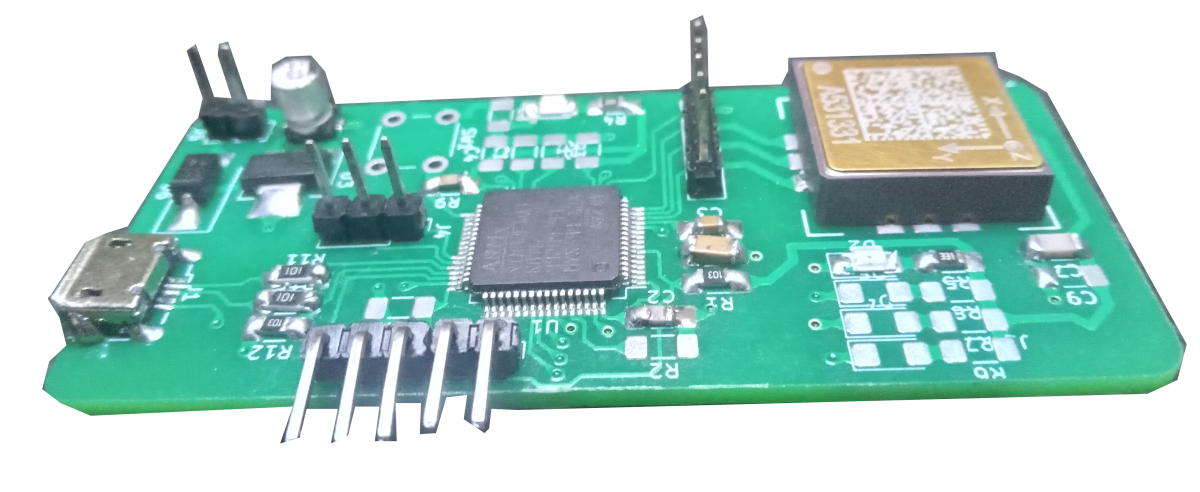
\includegraphics[width=0.8\textwidth,right]{images/vibs.png}
		\end{minipage}
	\end{figure}

	\raggedright

	\section{Project Repository}

	\begin{itemize}
		\item PCB Design: \url{https://github.com/VibrasticLab/wesel_monitoring/tree/master/circuit/mems_vibs}

		\item Firmware: \url{https://github.com/VibrasticLab/wesel_monitoring/tree/master/firmware}

		\item Interface: \url{https://github.com/VibrasticLab/wesel_monitoring/tree/master/interface/python/plot_test}

		\item Overall Repository: \url{https://github.com/VibrasticLab/wesel_monitoring/}
	\end{itemize}

	\section{Technical specification}
	\centering
	\begin{tabular}{lcr}
		\toprule
		Parts & Unit & Value \\
		\midrule
		Power voltage & $V$ & 3.7 to 7.4 \\
		Operation voltage & $V$ & 3.3 \\
		Main Chip & & STM32Fx LQFP64 \\
		Storage & & Internal EEPROM \\
		Data Interface & & 115200 UART \\
		USB Interface & & Unavailable \\
		MEMS chip & & TE-830M1-0025 \\
		Sampling Frequency & kHz & 8000 \\
		\bottomrule
	\end{tabular}

	\raggedright

	\section{Schematic Design}

	\newpage
	\includepdf[pages=-,angle=-90]{images/mems_vibs_sch.pdf}

	\newpage
	\section{Unit Preview}
	\begin{figure}[h]
		\centering
		\begin{subfigure}{0.45\textwidth}
			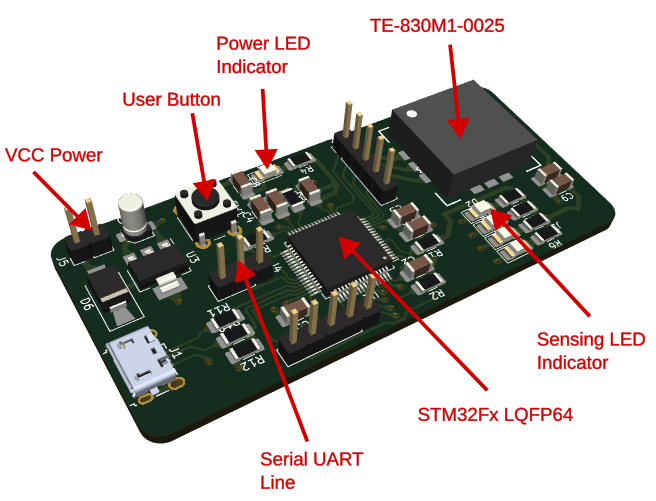
\includegraphics[width=\textwidth]{images/vibparts.png}
			\caption{Mockup}
		\end{subfigure}
		\begin{subfigure}{0.45\textwidth}
			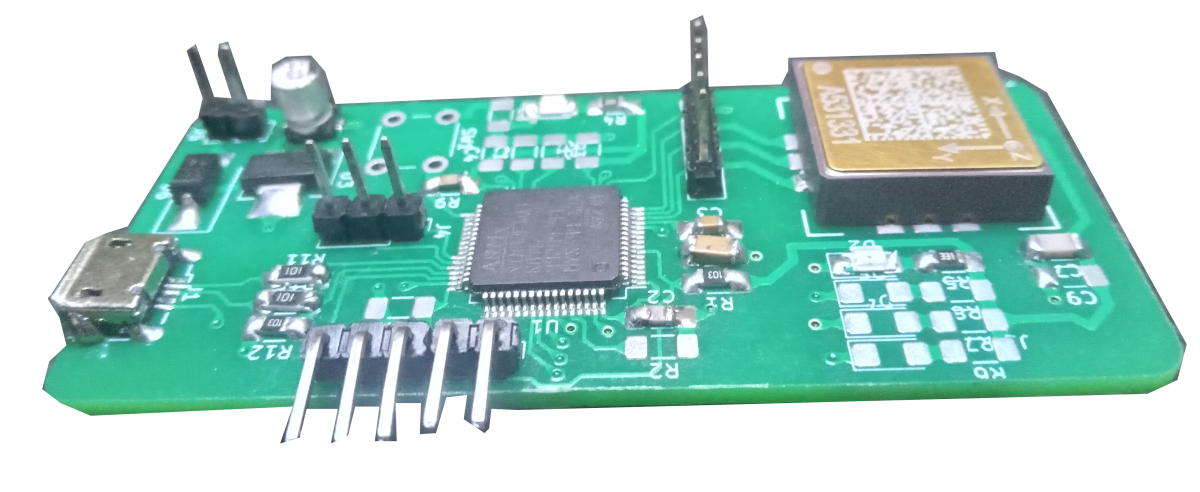
\includegraphics[width=\textwidth]{images/vibs.png}
			\caption{Actual}
		\end{subfigure}
	\end{figure}

	\section{Unit Testing}

	\subsection{Testing Diagram}

	\begin{figure}[h]
		\centering
		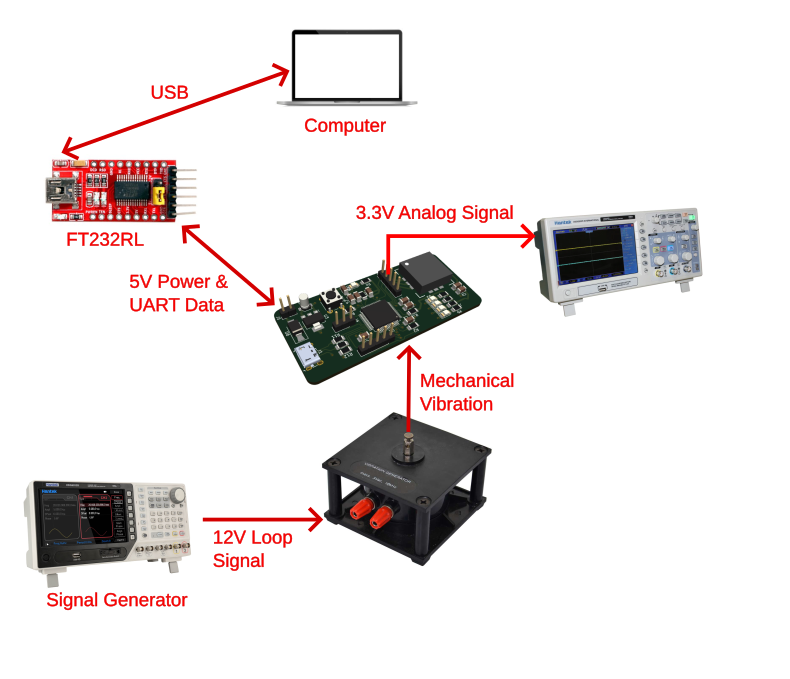
\includegraphics[width=0.75\textwidth]{images/testing.png}
		\caption{Diagram}
	\end{figure}

	\newpage
	\subsection{Testing Setup}

	\begin{figure}[h]
		\centering
		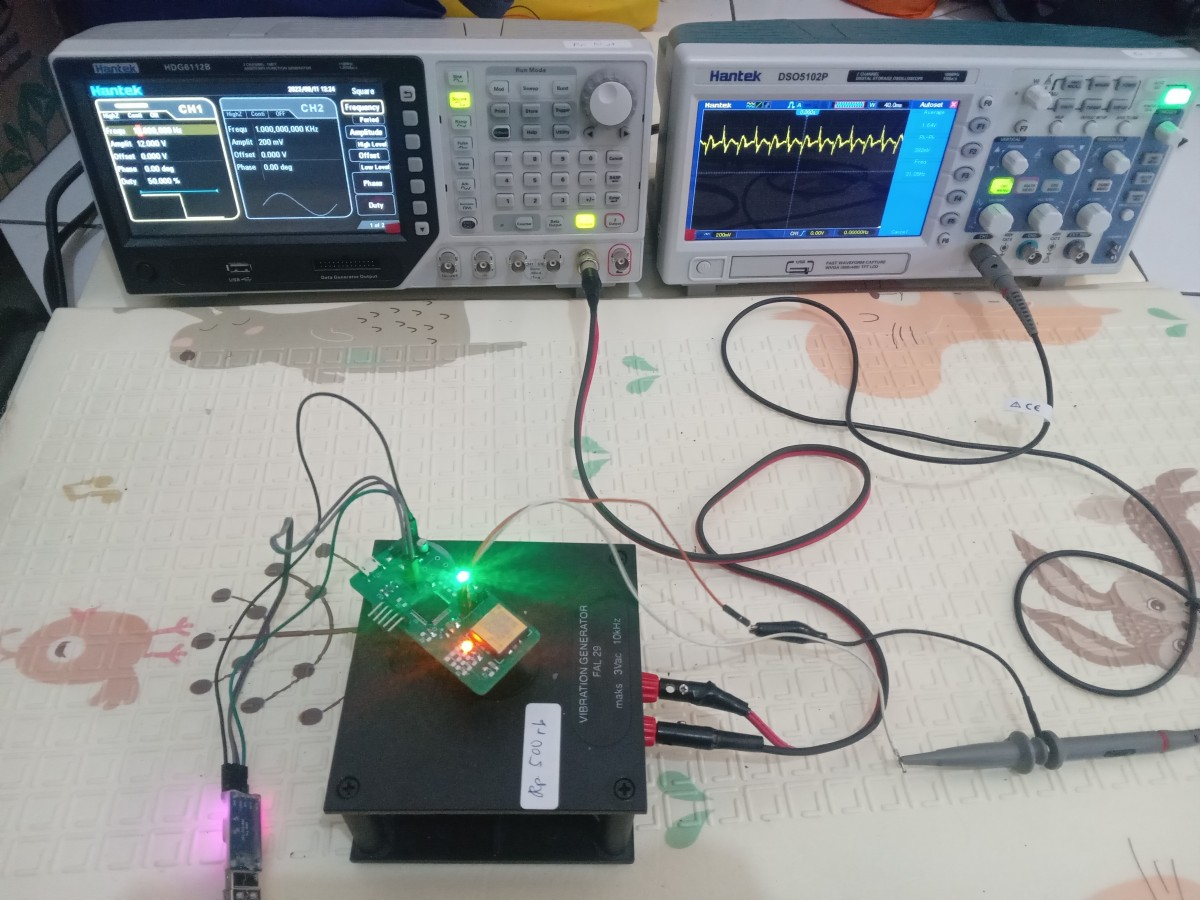
\includegraphics[width=0.65\textwidth]{images/testactual.jpg}
		\caption{Testing}
	\end{figure}

	\section{Interface}

	Interface prototype summary:
	\begin{itemize}
		\item Written for Python 3.6+ using Tkinter, Numpy, and Matplotlib.
		Planned to be enhanced with Tensorflow or Scikit-Learn.

		\item Fast Serial data using PySerial and compatible both Windows or Unix drivers.
	\end{itemize}
		\begin{figure}[h]
		\centering
		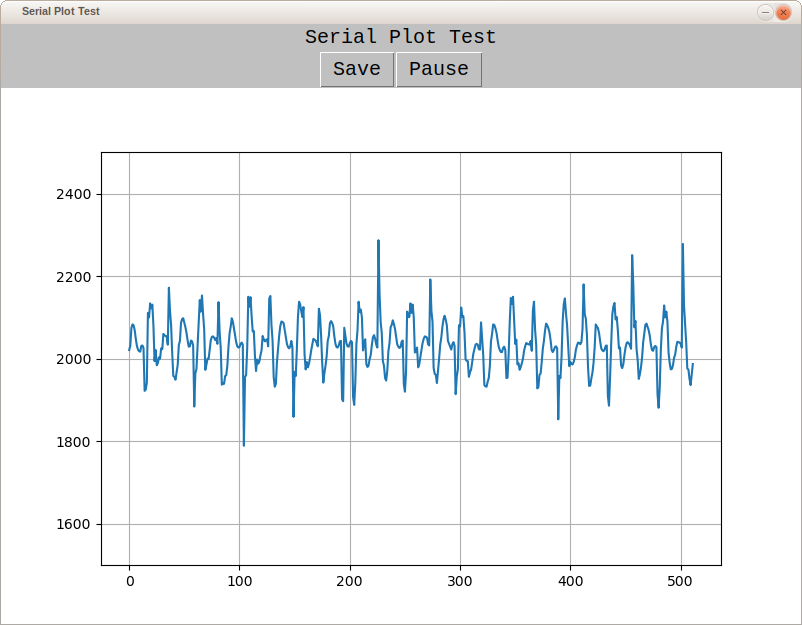
\includegraphics[width=0.6\textwidth]{images/protoiface.png}
		\caption{Python Interface}
	\end{figure}

\end{document}
